
%(BEGIN_QUESTION)
% Copyright 2012, Tony R. Kuphaldt, released under the Creative Commons Attribution License (v 1.0)
% This means you may do almost anything with this work of mine, so long as you give me proper credit

If the pulling force exerted on the end of the rope in this pulley system is 8 pounds, how much upward pulling force is exerted on the mass by the lower pulley?

$$\includegraphics[width=15.5cm]{i02628x01.eps}$$

Calculate the amount of work done in lifting the mass 3 feet while pulling on the rope with 8 pounds of force.

\underbar{file i02628}
%(END_QUESTION)





%(BEGIN_ANSWER)

With 8 pounds of tension in the cable, and {\it four} cables pulling upward on the lower pulley assembly, the total upward force exerted on the mass will be four times the tension, or 32 pounds.

\vskip 10pt

With a mechanical advantage of 4:1, the mass moves $1 \over 4$ the distance that the rope is pulled.  So, if the mass moves 3 feet, the rope must be pulled 12 feet.  This gives the following values for work done (calculated either at the mass or at the rope's end, yields the same result):

\vskip 10pt

$$W = F x = (8 \hbox{ lb}) (12 \hbox{ ft}) = 96 \hbox{ ft-lb \hskip 20pt (calculated at rope's end)}$$

$$W = F x = (32 \hbox{ lb}) (3 \hbox{ ft}) = 96 \hbox{ ft-lb \hskip 20pt (calculated at mass)}$$

%(END_ANSWER)





%(BEGIN_NOTES)


%INDEX% Machine, pulley
%INDEX% Machine, mechanical advantage
%INDEX% Physics, energy, work, power: calculating work and power

%(END_NOTES)


